\documentclass{cms-kurs}
\lstset{language=[LaTeX]TeX,
  morekeywords={onslide,pause,subtitle,pgfpagesuselayout,mode,
    maketitle,titlepage,institute,titlegraphic,subject,keywords,
    tableofcontents,AtBeginSection,uncover,visible,invisible,only,
    alt,temporal,alert,usetheme,setbeamertemplate,tikz,draw, setbeamerfont,
    textcolor,color,includegraphics,frametitle}}

\newenvironment{slide}
  {\begin{frame}[fragile,environment=slide]}
  {\end{frame}}

\begin{document}

\title{In-Depth: Präsentationen mit \LaTeX{}}
\author{dbo}
\date{2018-09-08}

\maketitle{}

\begin{frame}
  \frametitle{Agenda}

  \onslide<+->

  \vfill

  \begin{block}{Ziele}
    \begin{itemize}
    \item Eine schnelle Einführung in Präsentationen mit \LaTeX{}
    \item \emph{Keine} umfassende Einführung in \LaTeX{}
    \end{itemize}
  \end{block}

  \vfill

  \onslide<+->

  \begin{block}{Vorgehen}
    \begin{itemize}
    \item Zuerst gibt es \emph{viele} Informationen zum Thema
    \item Danach soll es praktisch werden
    \end{itemize}
  \end{block}

  \bigskip{}

  \onslide<+->

  Fast alle der folgenden Folien sind aus dem Kurs \emph{Wissenschaftliches
    Arbeiten mit \LaTeX} von Tom~Hanika und Daniel~Borchmann, HTW 2016,
  cc-by-sa.

\end{frame}

\section{\LaTeX{} Grundbegriffe}

\subsection{Philosophie}

\begin{frame}
  \frametitle{Was genau ist eigentlich \LaTeX?}

  \onslide<+->

  \begin{itemize}
  \item Ein freies System zum Setzen komplexer Dokumente
  \item Vor allem im akademischen Bereich verbreitet
  \item \emph{Kein} WYSIWYG!, anfänglich sehr steile Lernkurve
  \item Automatischer Textsatz
  \item Teilweise mit Charme der 1980er
  \item Ausprache: ,la-tech‘
  \end{itemize}

\end{frame}

\begin{frame}
  \frametitle{\LaTeX{} als Markup-Sprache}

  \onslide<+->

  \LaTeX{} ist eine \emph{Markupsprache}, d.h.~aus einem \emph{\LaTeX-Dokument}
  wird durch einen \emph{\LaTeX-Compiler} (\texttt{pdflatex}) das eigentliche
  Dokument erzeugt.

  \onslide<+->

  \begin{block}{Vorteile}
    \begin{itemize}
    \item \textbf{Trennung von Inhalt und Form}: beim Schreiben
      Konzentration auf Inhalt, die Formatierung übernimmt \LaTeX{} (im
      Idealfall \dots)
    \item Einheitlichkeit und Anpassbarkeit
    \item Versionkontrolle der Quelldateien
    \end{itemize}
  \end{block}

  \onslide<+->

  \begin{block}{Nachteile}
    \begin{itemize}
    \item Ungewohnte Arbeitsweise, steile Lernkurve
    \item Manuelle Mikroformatierung schwierig
    \item ausgefallene Layouts nur schwer realisierbar
    \end{itemize}
  \end{block}

\end{frame}

\begin{frame}
  \frametitle{\LaTeX{}-\texttt{beamer}}

  \onslide<+->

  \begin{columns}
    \begin{column}{0.7\linewidth}
      \begin{itemize}
      \item \LaTeX-\texttt{beamer} ist eine Dokumentenklasse für das Erstellen von
        Präsentationen mit \LaTeX
      \item Entwickelt von Till Tantau, weiter betreut von Joseph Wright and
        Vedran Miletić
      \item Weit verbreitet in der akademischen Welt (aber kaum darüber hinaus
        \dots)
      \item Aussehen der Präsentationen ähnlich zu anderen Systemen, meist aber
        etwas \enquote{statischer}
      \end{itemize}
    \end{column}
    \begin{column}{0.3\linewidth}
      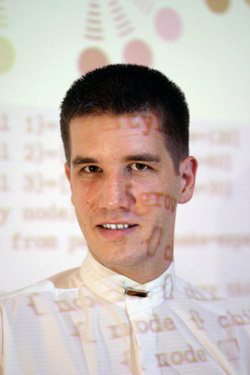
\includegraphics[width=.9\linewidth,keepaspectratio]{img/till-tantau}
      \rotatebox{90}{%
        \scalebox{0.3}{\url{http://www.tcs.uni-luebeck.de/mitarbeiter/tantau/}}}
    \end{column}
  \end{columns}

\end{frame}

\subsection{Grundlegendes Markup}

\begin{frame}[fragile]
  \frametitle{Allgemein Struktur eines \LaTeX{}-Dokuments}

  \onslide<+->

  \begin{itemize}
  \item Text im \emph{Dokumentenkörper} zwischen \lstinline|\begin{document}|
      und \lstinline|\end{document}|
  \item Textformatierung dazwischen \enquote{fast} beliebig, Text wird
    automatisch gesetzt (es gibt hier Ausnahmen …)
  \item Sonderfall: \emph{Kommandos} und \emph{Umgebungen}
  \end{itemize}

\end{frame}

\begin{slide}
  \frametitle{Abschnitte}

  \onslide<+->

  Abschnitte werden wie \LaTeX\ üblich mit \lstinline{\section}, \dots\ angelegt

\begin{lstlisting}
\section{Overlays}
\end{lstlisting}

  \onslide<+->

  \begin{itemize}
  \item Je nach Theme wird dies dann in den Kopf- oder Fußzeilen der Folien
    angezeigt.
  \item Werden automatisch im Inhaltsverzeichnis eingefügt.
  \end{itemize}

\end{slide}

\begin{slide}
  \frametitle{Inhaltsverzeichnis}

  \onslide<1->

  Einfach wie üblich mit
\begin{lstlisting}
\tableofcontents
\end{lstlisting}

  \onslide<2->{\tableofcontents}

\end{slide}

\begin{slide}
  \frametitle{Inhaltsverzeichnis}

  \onslide<1->

  Optionen sind auch möglich
\begin{lstlisting}
\tableofcontents[currentsection]
\end{lstlisting}

  \onslide<2->{\tableofcontents[currentsection]}

\end{slide}

\begin{slide}
  \frametitle{Inhaltsverzeichnis}

  \onslide<+->

\begin{lstlisting}
\AtBeginSection{%
  \tableofcontents[currentsection]
}
\end{lstlisting}
  zeigt bei jedem neuen Abschnitt an, wo man sich gerade in der Präsentation befindet.

\end{slide}

\begin{frame}[fragile]
  \frametitle{Aufzählungen}

  \LaTeX\ stellt standardmäßig drei Aufzählungstypen zur Verfügung%

  \onslide<+->

  \begin{enumerate}
  \item<+-> \lstinline{itemize} für unnummerierte Aufzählungen
  \item<+-> \lstinline{enumerate} für nummerierte Aufzählungen
  \item<+-> \lstinline{description} für Definitionslisten
  \end{enumerate}

  \onslide<+->

  \begin{Beispiel}
    \begin{columns}
      \begin{column}{0.4\linewidth}
\begin{lstlisting}
\begin{itemize}
\item Eins
\item Zwei
\item Drei
\end{itemize}
\end{lstlisting}
      \end{column}
      \onslide<+->
      \begin{column}{0.4\linewidth}
        \begin{itemize}
        \item Eins
        \item Zwei
        \item Drei
        \end{itemize}
      \end{column}
    \end{columns}
  \end{Beispiel}

\end{frame}

\begin{frame}[fragile]
  \frametitle{\textbf{Fett}, \textit{Kursiv} und \textsc{Ähnliches}}

  \onslide<+->

  Für das Markup einzelner Wörter oder Sätze stehen die folgenden Kommandos zur
  Verfügung: \bigskip

  \centering
  \begin{tabular}[c]{lcl}
    \lstinline!\textbf{Text}! & $\leadsto$ & \textbf{Text}\\
    \lstinline!\textsc{Text}! & $\leadsto$ & \textsc{Text}\\
    \lstinline!\emph{Text}!   & $\leadsto$ & \emph{Text}\\
    \lstinline!\textsf{Text}! & $\leadsto$ & \textsf{Text}\\
    \lstinline!\textit{Text}! & $\leadsto$ & \textit{Text}\\
    \lstinline!\textnormal{Text}! & $\leadsto$ & \textnormal{Text}\\
    \lstinline!\textrm{Text}! & $\leadsto$ & \textrm{Text}\\
    \lstinline!\textsl{Text}! & $\leadsto$ & \textsl{Text}\\
    \lstinline!\texttt{Text}! & $\leadsto$ & \texttt{Text}\\
  \end{tabular}

\end{frame}

\begin{frame}[fragile]
  \frametitle{Schriftgröße}

  \onslide<+->

  Schriftgrößen werden \emph{logisch} angegeben:

  \onslide<+->

  \begin{center}
    \begin{tabular}[c]{cc}
      \lstinline!\tiny Text!         & \tiny Text \\
      \lstinline!\scriptsize Text!   & \scriptsize Text \\
      \lstinline!\footnotesize Text! & \footnotesize Text \\
      \lstinline!\small Text!        & \small Text \\
      \lstinline!\normalsize Text!   & \normalsize Text \\
      \lstinline!\large Text!        & \large Text \\
      \lstinline!\Large Text!        & \Large Text \\
      \lstinline!\LARGE Text!        & \LARGE Text \\
      \lstinline!\huge Text!         & \huge Text \\
      \lstinline!\Huge Text!         & \Huge Text \\
    \end{tabular}
  \end{center}

  \onslide<+->

  Manuelle Größeneinstellung auch möglich (\lstinline!graphicx!)

\end{frame}

\begin{frame}[fragile]
  \frametitle{Farben}

  \onslide<+->

  Farben werden durch das Paket \lstinline{xcolor} bereitgestellt.

  \onslide<+->

\begin{lstlisting}
\usepackage{xcolor}
\textcolor{blue}{Blauer Text}
\textcolor{green}{Gruener Text}
\textcolor{red!50!blue}{Text blau-rot gemischt}
\color{gray} Alles, was jetzt noch kommt ist grau
\end{lstlisting}

  wird zu\onslide<+->

  \textcolor{blue}{Blauer Text}
  \textcolor{green}{Grüner Text}
  \textcolor{red!50!blue}{Text blau-rot gemischt}
  \color{gray} Alles, was jetzt noch kommt ist grau

\end{frame}

\begin{frame}[fragile]
  \frametitle{Bilder einbinden}

  \onslide<+->

  \begin{itemize}
  \item Einbinden von Graphiken in \LaTeX\ mit Hilfe des Pakets \texttt{graphicx}
  \item Befehl
\begin{lstlisting}
\includegraphics[\textit{Optionen}]%
  {\textit{Bildname}}
\end{lstlisting}
  \end{itemize}

  \onslide<+->

  \begin{Beispiel}
\begin{lstlisting}
\centerline{%
  
\includegraphics[width=0.3\linewidth]{bild.jpg}}
\end{lstlisting}

    ergibt

    \centerline{
\includegraphics[width=0.3\linewidth]{img/bild.jpg}}
  \end{Beispiel}

\end{frame}

\section{\LaTeX{} \texttt{beamer}}

\subsection{Folien erstellen}

\begin{slide}
  \frametitle{Frames}

  \onslide<+->

  Einzelne Folien werden mit \lstinline!\begin{frame}! \dots \lstinline!\end{frame}!
  erzeugt:
\begin{lstlisting}
\begin{frame}
  \frametitle{Frames}

  \dots

\end{frame}
\end{lstlisting}

  \onslide<+->

  Hinter \lstinline!\begin{frame}! können noch Optionen in \lstinline![...]!
    angegeben werden:
  \begin{itemize}
  \item \lstinline!label=$\textit{name}$!, um einzelnen Folien Label zu geben
  \item \lstinline{fragile}, falls die Folie \lstinline{verbatim}-Text oder
    Listings enthält
  \item \lstinline{plain}, falls die Folie keine Kopf- und Fußzeile haben soll
  \end{itemize}

\end{slide}

\begin{slide}
  \frametitle{Handouts}

  \onslide<+->

  Mit
\begin{lstlisting}
\documentclass[handout]{beamer}
\mode<handout>{%
  \usepackage{pgfpages}
  \pgfpagesuselayout{2 on 1}%
    [a4paper,border shrink=5mm]
}
\end{lstlisting}

  \onslide<+->

  Es sind dann eventuell kleine Anpassungen im Dokument nötig, meist bei den
  Overlays:
\begin{lstlisting}
\onslide<+| handout:0>
\end{lstlisting}

\end{slide}

\subsection{Strukturierungen}

\begin{slide}
  \frametitle{Titelfolie}

  Mit
\begin{lstlisting}
\frame{\titlepage}
\frame[plain]{\titlepage}
\frame[plain]{\maketitle}
\maketitle
\end{lstlisting}

  \onslide<+->

  Die Kommandos \lstinline{\author}, \lstinline{\title}, \lstinline{\subtitle},
  \lstinline{\date} funktionieren wie gewohnt.

  \onslide<+->

  Darüber hinaus gibt es noch \lstinline{\institute}, \lstinline{\titlegraphic},
  \lstinline{\subject}, \lstinline{\keywords}.

\end{slide}

\begin{slide}
  \frametitle{Blöcke}

  \onslide<+->

  Einträge auf einer Folie können in \emph{Blöcken} gruppiert werden:

\begin{lstlisting}
\begin{block}{Titel}
  Text Text Text
\end{block}
\end{lstlisting}

  \onslide<+->

  \medskip{}

  \begin{block}{Titel}
    Text Text Text
  \end{block}

  \medskip{}

  \onslide<+->

  Je nach Theme können die Blöcke auch Schatten haben:

  \medskip{}

  \setbeamertemplate{blocks}[rounded][shadow=true]
  \begin{block}{Titel}
    Text Text Text
  \end{block}
  \setbeamertemplate{blocks}[rounded][shadow=false]

  \onslide<+->

  Vordefinierte Blöcke: \texttt{Satz}, \texttt{Beweis}, \texttt{Beispiel}, \dots
\end{slide}

\subsection{Einblendungen}

\begin{slide}
  \frametitle{Overlay-Kommandos}

  \onslide<+->

  Beamer stellt verschiedene Möglichkeiten bereit, \textit{overlays} zu
  erzeugen, welche dann als aufeinander folgenden Seiten im erzeugten Dokument
  dargestellt werden:

  \onslide<+->

  \begin{itemize}
  \item \lstinline{\pause}
  \item \lstinline{\onslide}
  \item \lstinline{\uncover}
  \item \lstinline{\visible}, \lstinline{\invisible}
  \item \lstinline{\only}
  \item \lstinline{\alt}, \lstinline{\temporal}, \lstinline{onlyenv},
    \lstinline{overprint}, \lstinline{altenv}, \lstinline{overlayarea}, \dots
  \end{itemize}

  \onslide<+->

  Mit Hilfe von \lstinline{\pause} können einzelne Abschnitte nacheinander aufgedeckt
  werden.

  \onslide<+->

  Alle anderen Anweisungen werden durch \emph{Overlay-Spezifikationen} gesteuert.

\end{slide}

\begin{slide}
  \frametitle{Overlay-Spezifikationen}

  \onslide<+->

  \begin{Beispiele}
\begin{lstlisting}
\onslide<2-4>{Ich bin ein Text}
\end{lstlisting}
    erscheint auf Folien 2 bis 4 (inklusive); Text nimmt aber Platz ein, auch wenn er
    nicht gezeigt wird
    \onslide<+->
\begin{lstlisting}
\onslide<2->{Ich bin noch ein Text}
\end{lstlisting}
    erscheint auf Folie 2 und bleibt bis zum Ende
    \onslide<+->
\begin{lstlisting}
\onslide<-4>{Text Text Text}
\end{lstlisting}
    erscheint von Anfang an, verschwindet dann aber auf Folie 5
    \onslide<+->
\begin{lstlisting}
\onslide<2->
Noch mehr Text Text Text\dots
\end{lstlisting}
    Alles nach dieser Anweisung wird erst ab Folie 2 angezeigt.
  \end{Beispiele}

\end{slide}

\begin{slide}
  \frametitle{Overlay-Spezifikationen}

  \onslide<+->

  \begin{block}{\textcolor{red}{Problem}}
    Die explizite Angabe von Folien-Nummern ist unhandlich.
  \end{block}

  \onslide<+->

  Aber es geht auch ohne!

  \onslide<+->

  \begin{Beispiele}
\begin{lstlisting}
\onslide<+->
\end{lstlisting}
    Alles, was dieser Anweisung folgt, wird auf der \emph{nächsten} Folie aufgedeckt.
    \onslide<+->
\begin{lstlisting}
\onslide<+->{Teeeeeeeext}
\end{lstlisting}
    Der Text wird auf der folgenden Folie angezeigt.
    \onslide<+->
\begin{lstlisting}
\onslide<.->{Texxxxxxxxxt}
\end{lstlisting}
    Der Text wird auf der \emph{aktuellen} Folie mit angezeigt. (sinnvoll mit
    \lstinline{\alert} statt \lstinline{\onslide})
  \end{Beispiele}

\end{slide}

\begin{slide}
  \frametitle{Weitere Anweisungen mit Overlay-Spezifikationen}

  \onslide<+->

  \begin{Beispiele}
\begin{lstlisting}
\alert<2>{ACHTUNG!}
\end{lstlisting}
    Zeigt \alert<.>{ACHTUNG!} auf Folie 2 hervorgehoben an.
    \onslide<+->
\begin{lstlisting}
\item<+-> Noch ein Text ohne Sinn
\end{lstlisting}
    Zeigt den entsprechenden Punkt auf der nächsten Folie an
    \begin{overprint}[\linewidth]
      \onslide<+| handout:0>
\begin{lstlisting}
\begin{itemize}
\item<+-> Foo
\item<+-> Bar
\item<+-> Baz
\end{itemize}
\end{lstlisting}
      \onslide<+-| handout:1>
\begin{lstlisting}
\begin{itemize}[<+->]
\item Foo
\item Bar
\item Baz
\end{itemize}
\end{lstlisting}
    \end{overprint}
  \end{Beispiele}

\end{slide}

\subsection{Diverses}

\begin{frame}[fragile]
  \frametitle{Farben und Aussehen einstellen}

  \onslide<+->

  \LaTeX-\texttt{beamer} bietet viele Möglichkeiten, das Aussehen anzupassen.
  \onslide<+->
\begin{lstlisting}
\usetheme{CambridgeUS}
\setbeamertemplate{blocks}[rounded][shadow=false]
\setbeamertemplate{items}{\raisebox{0.3ex}{%
 \tikz[scale=0.13]%
  \draw[fill] (0,0) -- (0,1) -- (0.9,0.5) -- cycle;}}
\setbeamertemplate{navigation symbols}{}
\setbeamertemplate{footline}{}
\setbeamerfont{title}{series=\bfseries}
\end{lstlisting}
  \onslide<+->

  Viel mehr in der Dokumentation!

\end{frame}

\begin{frame}[fragile]
  \frametitle{Don't Panic!}

  \onslide<+->

  Es mag jetzt alles ziemlich Angst einflößend wirken, was man alles wissen
  muss, um \LaTeX{} zu benutzten, aber \ldots

  \onslide<+->

  \begin{center}
    \Large%
    \textbf{Um \LaTeX{} nutzen zu können,\\ muss man nicht alles über \LaTeX{}
      wissen!}
  \end{center}

  Ein solides Grundwissen reicht meist aus.

  \onslide<+->

  Weitere Hilfe:

  \begin{itemize}
  \item \verb|texdoc «Paket-oder-Klasse»|
  \item CTAN (Comprehensive \TeX{} Archive Network, \url{https://ctan.org})
  \item Im allgemeinen das INTERNET (Mailinglisten, Foren, \dots)
  \item Die \LaTeX-Sprechstunde der FSFW
    (\url{https://fsfw-dresden.de/sprechstunde})
  \end{itemize}

\end{frame}

\end{document}
